\documentclass[
  a4paper,            % DIN A4
  DIV=10,             % Schriftgröße und Satzspiegel    
  %12pt
  oneside,            % einseitiger Druck
  %fleqn
  %draft,             % Fehler in overfull checken
  BCOR=5mm,           % Bindungskorrektur
  parskip=half,       % Halber Abstand zwischen Absätzen
  numbers=noenddot    % Kein Punkt hinter Kapitelnummern
]{scrartcl}
\usepackage{style/style}
\usepackage{graphicx}
\graphicspath{{img/}}
 
%%%%% Konfigurierung der Kopfzeile %%%%%
\lohead{\today}
\chead{Handout}
%%\rohead{\includegraphics[scale=2]{LogoTI1.png}}	% Braucht keine Umgebung

%\setlength{\headsep}{1.5cm}
 \setlength{\headheight}{2.07\baselineskip} 

%%%%% Konfigurierung der Fußzeile %%%%%
\cfoot{\pagemark}                       % Nummerierung  der Seitenzahlen
\lofoot{}
\rofoot{}


%%%%%% Beginn of document %%%%%
\begin{document}
%%%%% TitlePage %%%%%
\pagenumbering{gobble}			    % Nummerierung auslassen auf dieser Seite
\begin{titlepage}
	\centering
	\text{}\vspace{3cm} \\
	{\scshape\LARGE Funktion und Arbeit von Betriebsräten \par}
	\vspace{1cm}
	{\scshape\Large 
		Handout zur Präsentation \par}
	\vspace{1.5cm}
	{\huge\bfseries \par}
	\vspace{2cm}
	{\Large\itshape     	
            Thanh-Viet Nguyen \\
            \par}
\vfill
\begingroup
\leftskip2.5cm		
        \textbf {} %%Unterzeile
\endgroup
\end{titlepage}

%%%%% Table of contents %%%%%%
    \tableofcontents
    % \listoffigures
    % \listoftables
\clearpage

%%%%% Beginn of the main TEXT %%%%
\pagenumbering{arabic} 			       %Nummerierung fortsetzen
%\chapternumbering{Roman}

\section{Einleitung} \label{sec:intro}
    Die Mitbestimmung im Betrieb ist in den letzten Jahrzehnten immer wichtiger geworden und deshalb auch gesetzlich geregelt. Sie bezeichnet die Teilnahme der Arbeitnehmer bzw. deren Vertreter an den Entscheidungsprozessen innerhalb eines Unternehmens. So wird denjenigen, deren Arbeits- und Lebensverhältnisse von den Entscheidungen anderer abhängig sind, eine Einfluss- und Gestaltungsmöglichkeit gewährleistet. 
\newline
Die betriebliche Mitbestimmung, wie sie durch den Betriebsrat repräsentiert wird, gibt den Arbeitnehmern die rechtliche Möglichkeit mitzureden, wenn es um betriebliche Belange geht.
\newline
Arbeitnehmer befinden sich durch das Arbeitsverhältnis in einer Abhängigkeit zu ihrem Arbeitgeber. Diese Abhängigkeit hat einen Einfluss nicht nur auf die Arbeitsgestaltung, sondern im weiteren Sinne auch auf die Lebensweise und Lebensverhältnisse der Arbeitnehmer. 
\newline
Zwar sind Arbeitgeber aufgrund der rechtlichen Besitzverhältnisse grundsätzlich frei in ihren unternehmerischen Entscheidungen, diese sind allerdings durch die rahmengebende Gesetzgebung zur Mitbestimmung im Betrieb begrenzt. Dies dient dem Schutz der Arbeitnehmer und findet beispielsweise Anwendung in folgenden Bereichen:
\begin{itemize}
	\item Mitbestimmung bei der Arbeitsgestaltung und Rahmenbedingungen durch Vorschlagsrecht
	\item Anspruch auf Aufklärung zur auszuübenden Tätigkeit und damit verbundener Verantwortung
	\item Einhaltung des Arbeitsschutzes und der Beurteilung von Gefährdungen
	\item Recht der Arbeitnehmer auf Einsicht in die Personalakte
	\item Recht der Vertreter der Arbeitnehmer zur Mitbestimmung bei unternehmerischen Entscheidungen, wie
	\begin{itemize}
		\item Zeiterfassung der Arbeitnehmer
		\item Kontroll- und Bewertungssysteme der Arbeitnehmer
		\item Personalplanung
		\item Sozialplan und Interessenausgleich bei unternehmerischen Umstrukturierungen
		\item Einführung von Incentives und anderen Anreizsystemen
		\item Auswahl von Mitarbeitern und deren Ausscheiden durch Kündigung
		\item Ausgestaltung von Betriebsvereinbarungen
	\end{itemize}
\end{itemize}
\section{Funktion und Arbeit des Betriebsrats} 
    Zwar sind Arbeitgeber aufgrund der rechtlichen Besitzverhältnisse grundsätzlich frei in ihren unternehmerischen Entscheidungen, diese sind allerdings durch die rahmengebende Gesetzgebung zur Mitbestimmung im Betrieb begrenzt. Dies dient dem Schutz der Arbeitnehmer und findet beispielsweise Anwendung in folgenden Bereichen: 
\begin{itemize}
	\item Mitbestimmung bei der Arbeitsgestaltung und Rahmenbedingungen durch Vorschlagsrecht
	\item Anspruch auf Aufklärung zur auszuübenden Tätigkeit und damit verbundener Verantwortung
	\item Einhaltung des Arbeitsschutzes und der Beurteilung von Gefährdungen
	\item Recht der Arbeitnehmer auf Einsicht in die Personalakte
	\item Recht der Vertreter der Arbeitnehmer zur Mitbestimmung bei unternehmerischen Entscheidungen
	\begin{itemize}
		\item Zeiterfassung der Arbeitnehmer
		\item Kontroll- und Bewertungssysteme der Arbeitnehmer
		\item Personalplanung
		\item Sozialplan und Interessenausgleich bei unternehmerischen Umstrukturierungen
		\item Einführung von Insentives und anderen Anreizsystemen
		\item Auswahl von Mitarbeitern und deren Ausscheiden durch Kündigung
		\item Ausgestaltung von Betriebsvereinbarungen
	\end{itemize}
\end{itemize}
Die allgemeinen Aufgaben des Betriebsrats sind in Paragraf 80 Absatz 1 des Betriebsverfassungsgesetzes geregelt. Danach hat der Betriebsrat folgende allgemeine Aufgaben:
\begin{itemize}
	\item
	Die Beschäftigung im Betrieb zu fördern und zu sichern.
	\item
	Die Beschäftigung älterer Arbeitnehmerinnen und Arbeitnehmer im Betrieb zu fördern.
	\item 
	Der Betriebsrat hat darüber zu wachen, dass die zugunsten der Arbeitnehmer geltenden Gesetze, Verordnungen und Unfallverhütungsvorschriften, Tarifverträge und Betriebsvereinbarungen vom Arbeitgeber eingehalten werden.
	\item
	Maßnahmen des Arbeitsschutzes und des betrieblichen Umweltschutzes zu fördern.
	\item
	Maßnahmen, die dem Betrieb und der Belegschaft dienen, beim Arbeitgeber zu beantragen. Die Durchsetzung der tatsächlichen Gleichstellung von Frauen und Männern zu fördern, insbesondere bei der Einstellung, Beschäftigung, Aus-, Fort- und Weiterbildung und dem beruflichen Aufstieg und die Vereinbarkeit von Familie und Erwerbstätigkeit zu fördern.
	\item 
	Anregungen von Arbeitnehmerinnen und Arbeitnehmern und der Jugend- und Auszubildendenvertretung entgegenzunehmen und, falls sie berechtigt erscheinen, durch Verhandlungen mit dem Arbeitgeber auf eine Erledigung hinzuwirken; er hat die betreffenden Arbeitnehmer über den Stand und das Ergebnis der Verhandlungen zu unterrichten.
	\item
	Die Eingliederung schwerbehinderter Menschen einschließlich der Förderung des Abschlusses von Inklusionsvereinbarungen nach § 166 des Neunten Buches Sozialgesetzbuch und sonstiger besonders schutzbedürftiger Personen zu fördern.
	\item
	Die Wahl einer Jugend- und Auszubildendenvertretung (JAV) vorzubereiten und durchzuführen und mit dieser zur Förderung der Belange der in § 60 Abs. 1 genannten Arbeitnehmer eng zusammenzuarbeiten; er kann von der Jugend- und Auszubildendenvertretung Vorschläge und Stellungnahmen anfordern.
	\item
	Die Integration ausländischer Arbeitnehmer im Betrieb und das Verständnis zwischen ihnen und den deutschen Arbeitnehmern zu fördern, sowie Maßnahmen zur Bekämpfung von Rassismus und Fremdenfeindlichkeit im Betrieb zu beantragen.
\end{itemize}


\section{Rechte des Betriebsrats} 
	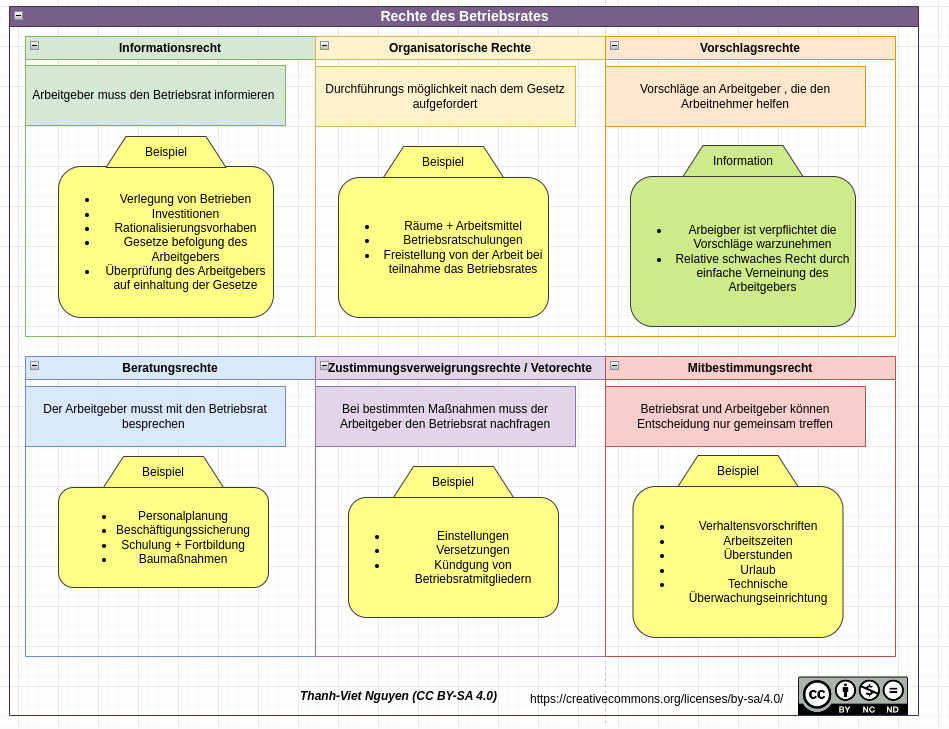
\includegraphics [width=15cm, height=10cm] {img/BetriebsratsRechte.png}
\begin{comment}
\begin{enumerate}
	\item 
	Informationsrechte
	\item 
	Vorschlagsrechte
	\item
	Beratungsrechte
	\item
	Zustimmungsverweigerungsrechte
	\item
	Mitbestimmungsrechte
	\item
	Organisatorische Rechte
	\item
	Sonstige Rechte
	\item
	Informations- und Unterrichtungsrechte
	\item
	Vorschlagsrechte
	\item
	Beratungsrechte
	\item
	Zustimmungsverweigerungsrechte
	\item
	Mitbestimmungsrechte
	\item
	Organisatorische Rechte
	\item
	Sonstige Rechte
	\item
	Rechte bei der Kündigung eines Arbeitnehmers
	\item
	Recht auf Einhaltung einer Betriebsvereinbarung oder Regelungsabrede
	\item
	Recht auf Einhaltung eines Einigungsstellenspruchs
	\item
	Unterlassungsanspruch bei Störung oder Behinderung der Betriebsratsarbeit
	\item
	Rechte bei groben Verstößen des Arbeitgebers (§ 23 Abs. 3 BetrVG)
	\item
	Recht auf Entfernung betriebsstörender Arbeitnehmer
	\item
	Hinzuziehungs- und Teilnahmerechte
\end{enumerate}
\end{comment}

\section{Weitere Informationen}
	\subsection*{Betriebsrätemodernisierungsgesetz}
{
	Erleichterungen nach dem Betriebsrätemodernisierungsgesetz: 
	Mit dem Betriebsrätemodernisierungsgsetz in 2021 ist die Gründung von Betriebsräten erleichtert worden, die Mitbestimmungsrechte bestehender Betriebsräte wurden erweitert. Konkret bedeutet das u.a.: Das vereinfachte Wahlverfahren zur Gründung eines Betriebsrats gilt jetzt auch in Unternehmen mit bis zu 100 Beschäftigten, statt wie früher nur bis zu einer Belegschaft von 50 Beschäftigten. Und demnach sind nur in Unternehmen mit mehr als 20 Beschäftigten zwei Unterschriften für Wahlvorschläge erforderlich. In Firmen mit weniger als 20 Beschäftigten werden gar keine Unterschriften von Beschäftigten mehr benötigt, um einen Betriebsrat zu gründen.
}
Weitere Gesetze und Regelungen: Der Betriebsrat muss für die Einhaltung von Gesetzen, Grundrechten und Arbeitsverträgen sorgen: Dazu gehören Arbeitsgesetze, Tarifverträge sowie die Arbeitsverträge, die für die Beschäftigten gelten. Der Betriebsrat hat darüber zu wachen, dass die zugunsten der Arbeitnehmer geltenden Gesetze, Verordnungen und Unfallverhütungsvorschriften, Tarifverträge und Betriebsvereinbarungen vom Arbeitgeber eingehalten werden. (Paragraf 80 Absatz 1)
\newline 
Die Rechte und Grundsätze der Zusammenarbeit von Betriebsräten mit dem Arbeitgeber sind im Betriebsverfassungsgesetz festgeschrieben. Dort sind auch die Arbeitsfelder genannt, in denen er mitbestimmen darf:
\newline 
Größe des Betriebsrats: Wenn es genug Wahlberechtigte und wählbare Beschäftigte gibt und sich genug Kandidaten finden, kann gewählt werden, auch wenn die Mehrheit noch nicht überzeugt ist. Bei bis zu 20 Wahlberechtigten wird eine Person gewählt, bei bis zu 50 drei, bei bis zu 100 sind es fünf, bei 200 sind es sieben und bei bis zu 400 Wahlberechtigten sind es neun Betriebsratsmitglieder.


\newpage

\section{Fazit} %%\label{conclusion}
  Folgende Ziele sollen durch die betriebliche Mitbestimmung erreicht werden:
\begin{figure} [H]
	\centering
	\includegraphics[width=0.7\linewidth]{"img/Vorteile Der Mitbestimmung"}
	\caption{https://www.bwl-lexikon.de/app/uploads/mitbestimmung-im-betrieb-1.png}
	\label{fig:vorteile-der-mitbestimmung}
\end{figure}
\section{Quellen}
   \begin{itemize}
   	\item 
   	https://www.betriebsrat.com/wissen/betriebsrat/mitbestimmung
   	\item  
   	https://www.bwl-lexikon.de/wiki/mitbestimmung-im-betrieb/
	\item 
	https://www.verdi.de/themen/arbeit/++co++743d550e-7794-11ec-9146-001a4a16012a
	\item
	http://www.gesetze-im-internet.de/betrvg/index.html 
	\item 
	https://www.bwl-lexikon.de/wiki/mitbestimmungsrecht-des-betriebsrats/
\end{itemize}
%\section{References}

%\bibliographystyle{dinat}
%\bibliography{literature}

\clearpage
%\newpage
%\section{Anhang}

\end{document}